% ARCHITECTURE.tex — HC-91 Emulator architecture, with SysML-style diagrams.
% Build:  pdflatex -interaction=nonstopmode -halt-on-error ARCHITECTURE.tex
%         (run twice for the TOC / references)
\documentclass[11pt,a4paper]{article}

\usepackage[T1]{fontenc}
\usepackage[utf8]{inputenc}
\usepackage{lmodern}
\usepackage{amssymb}   % \blacklozenge, etc.
\usepackage[a4paper,margin=2.2cm,top=2.0cm,bottom=2.2cm]{geometry}
\usepackage{xcolor}
\usepackage{tikz}
\usepackage{enumitem}
\usepackage{booktabs}
\usepackage{array}
\usepackage{titlesec}
\usepackage[colorlinks=true,linkcolor=accent,urlcolor=accent,
            pdftitle={HC-91 Emulator Architecture},
            pdfauthor={hc91emu audit}]{hyperref}

% ---- TikZ libraries for SysML-style diagrams ----
\usetikzlibrary{positioning,fit,calc,backgrounds,shapes.geometric,
                shapes.misc,arrows.meta,chains,decorations.pathreplacing}

% ---- Palette ----
\definecolor{accent}{HTML}{1F4E79}
\definecolor{accent2}{HTML}{8C2D2D}
\definecolor{blockfill}{HTML}{EAF1F8}
\definecolor{blockfill2}{HTML}{FBEEEC}
\definecolor{actfill}{HTML}{F2F7E9}
\definecolor{statefill}{HTML}{FBF3D9}
\definecolor{portfill}{HTML}{2E2E2E}
\definecolor{linegray}{HTML}{555555}

\hypersetup{linkcolor=accent}

% ============================================================
%  SysML-style node/edge styles
% ============================================================
\tikzset{
  % --- Block Definition Diagram blocks ---
  sysml/.style={draw=accent, very thick, rounded corners=3pt, align=center,
                fill=blockfill, inner sep=5pt, font=\sffamily\small,
                minimum width=26mm, line cap=round},
  sysml2/.style={sysml, fill=blockfill2, draw=accent2},
  blocklabel/.style={font=\sffamily\footnotesize\itshape, text=accent!70!black},
  % --- composition (filled diamond at the WHOLE, draw from part to whole) ---
  composition/.style={very thick, draw=linegray,
                      {Diamond[fill=linegray,length=3.2mm,width=2.6mm]}-},
  aggregation/.style={very thick, draw=linegray,
                      {Diamond[fill=white,length=3.2mm,width=2.6mm]}-},
  % --- dependency / association ---
  depends/.style={-{Stealth[length=2.6mm]}, thick, draw=accent!70!black,
                  dashed},
  assoc/.style={thick, draw=linegray, -{Stealth[length=2.4mm,open]}},
  bus/.style={thick, draw=accent, double, double distance=1.4pt},
  % --- Internal Block Diagram proxy ports ---
  port/.style={draw=accent!70!black, fill=portfill, rectangle,
               minimum width=2.2mm, minimum height=2.2mm, inner sep=0pt},
  % --- Activity diagram nodes ---
  actstart/.style={circle, fill=black, draw=black, minimum size=4mm, inner sep=0pt},
  actend/.style={circle, draw=black, thick, fill=white, minimum size=5mm,
                 inner sep=0pt},
  actfinal/.style={circle, draw=black, thick, fill=black, minimum size=4mm,
                   inner sep=0pt},
  actnode/.style={draw=accent, thick, fill=actfill, rounded corners=4pt,
                  align=center, font=\sffamily\footnotesize, inner sep=4pt,
                  minimum height=6.5mm},
  actdec/.style={diamond, draw=accent2, thick, fill=blockfill2, aspect=1.7,
                 align=center, inner sep=2pt, font=\sffamily\scriptsize},
  actbar/.style={draw=linegray, very thick, fill=linegray,
                 minimum width=14mm, minimum height=1.2mm, inner sep=0pt},
  actflow/.style={-{Stealth[length=2.4mm]}, thick, draw=linegray},
  % --- State machine ---
  smstate/.style={draw=accent, thick, fill=statefill, rounded corners=6pt,
                  align=center, font=\sffamily\footnotesize, inner sep=4pt,
                  minimum width=24mm, minimum height=8mm},
  smstart/.style={circle, fill=black, draw=black, minimum size=4mm, inner sep=0pt},
  smfinal/.style={circle, draw=black, thick, fill=black, minimum size=4mm,
                  inner sep=0pt},
  smflow/.style={-{Stealth[length=2.4mm]}, thick, draw=linegray},
}

% small helper for a SysML block header (stereotype + name)
\newcommand{\blkhead}[2]{\textit{«#1»}\\[1pt]\textbf{#2}}

\titleformat{\section}{\Large\bfseries\sffamily\color{accent}}{\thesection}{0.7em}{}
\titleformat{\subsection}{\large\bfseries\sffamily\color{accent!85!black}}
            {\thesubsection}{0.6em}{}
\setlist[itemize]{leftmargin=*,itemsep=2pt,topsep=2pt}
\setlist[enumerate]{leftmargin=*,itemsep=2pt,topsep=2pt}

\renewcommand{\arraystretch}{1.18}

\title{\textbf{HC-91 Emulator — Architecture}\\[2pt]
       \large A source-code-level tour with SysML-style diagrams}
\author{Derived from a source audit of \texttt{cosmindxu/hc91emu}}
\date{}

\begin{document}
\sloppy
\maketitle
\thispagestyle{empty}

\begin{quote}\small\itshape
This document is the companion to \texttt{docs/ARCHITECTURE.md}. It re-states
the architecture of \texttt{hc91emu}---a cycle-accurate, dependency-free
emulator for the I.C.E.\ Felix HC-91 (a Romanian ZX Spectrum 48K clone) and the
wider HC family---and illustrates it with SysML-style diagrams: Block
Definition (BDD), Internal Block (IBD), Activity, State-Machine and Sequence
diagrams. File/line references are relative to the repository root.
\end{quote}

\tableofcontents
\vspace{4pt}\hrule height 0.4pt

% ============================================================
\section{What is being emulated}

\begin{center}
\begin{tabular}{@{}p{1.8cm}p{13.4cm}@{}}
\toprule
\textbf{Aspect} & \textbf{Emulated target} \\
\midrule
CPU    & Z80A / Romanian MMN80 clone @ 3.5\,MHz (3{,}500{,}000 T-states/s) \\
Video  & ULA: 256$\times$192 paper, 15 colours; rendered with border at 320$\times$240 \\
Frame  & 50\,Hz, \textbf{69{,}888 T-states/frame} (312 lines $\times$ 224 T) \\
Audio  & 1-bit beeper (ULA bit 4); AY-3-8912 PSG on the HC-128 \\
Memory & 16K ROM + 48K RAM (HC-91); 128K banked + AY (HC-128); disk + CP/M (HC-2000) \\
I/O    & ULA \texttt{0xFE}; Kempston \texttt{0x1F}; AY \texttt{0xFFFD/0xBFFFD}; i8272 \texttt{0x85/0x87} \\
\bottomrule
\end{tabular}
\end{center}

The HC-91 ROM differs from the Sinclair 48K ROM by only $\sim$50 bytes
(copyright banner + a small CP/M boot stub), so the machine is fully
48K-Spectrum software compatible---a fact the project leans on hard.

% ============================================================
\section{Repository layout}

\begin{center}\footnotesize
\begin{tabular}{ll}
\toprule
\textbf{Path} & \textbf{Role} \\
\midrule
\texttt{src/z80.[ch]}        & bus-callback Z80 core (no machine knowledge) \\
\texttt{src/machine.[ch]}    & memory map, I/O bus, frame loop, file dispatch \\
\texttt{src/video.c}         & beam-accurate renderer + ROM-font OCR \\
\texttt{src/wav.c}           & beeper $\rightarrow$ 44.1\,kHz WAV synthesis \\
\texttt{src/ay.c}            & AY-3-8912 PSG (HC-128) \\
\texttt{src/tape.c}          & \texttt{.tap/.tzx/.wav}: trap + pulse loader + SAVE \\
\texttt{src/fdc.[ch]}        & uPD765/i8272 floppy controller (HC-2000) \\
\texttt{src/snapshot.c}      & \texttt{.sna/.z80/.szx/.scr} load + save \\
\texttt{src/rzx.[ch]}        & RZX input record/replay (deterministic regression) \\
\texttt{src/keys.c}          & scheduled keyboard events, typing, joysticks \\
\texttt{src/disasm.[ch]}     & full-coverage Z80 disassembler \\
\texttt{src/debug.[ch]}      & scriptable monitor: bp/watch/step/trace \\
\texttt{src/inflate.[ch]}    & built-in DEFLATE/zlib inflater (SZX/RZX) \\
\texttt{src/png.c}           & minimal PNG writer (no deps) \\
\texttt{src/sdl.c}           & optional SDL2 frontend (\texttt{dlopen}'d at runtime) \\
\texttt{src/main.c}          & CLI driver: option parse, run loop, output \\
\texttt{src/zexrun.c}        & standalone CP/M harness for zexdoc/zexall \\
\midrule
\texttt{tests/}              & unit + integration tests, golden images, test-tap generators \\
\texttt{tools/}              & ROM/library fetchers, deb/Windows packaging \\
\texttt{.github/workflows/ci.yml} & download-free CI (build + ASan/UBSan) \\
\bottomrule
\end{tabular}
\end{center}

The whole emulator is $\sim$7{,}700 lines of C99 with \textbf{zero external
dependencies} (libc + \texttt{-ldl} for the optional SDL runtime binding).
PNG encoding, DEFLATE inflation, WAV writing and the SDL2 ABI slice are all
implemented in-tree.

% ============================================================
\section{Layered architecture (Block Definition Diagram)}

The design is a clean, dependency-pointing-downwards stack. The Z80 core sits
at the bottom and knows nothing about the machine; everything above plugs bus
behaviour into it through callbacks.

\begin{figure}[h]\centering
\resizebox{\textwidth}{!}{%
\begin{tikzpicture}[
  font=\sffamily\small,
  b/.style={sysml, minimum width=30mm, minimum height=13mm, inner sep=4pt},
  b2/.style={sysml2, minimum width=34mm, minimum height=13mm, inner sep=4pt},
]
  % --- Tier A: UX (top) ---
  \node[b2] (main) at (-4,5.2) {\blkhead{component}{CLI Driver}\\\scriptsize\texttt{main.c}};
  \node[b2] (sdl)  at ( 4,5.2) {\blkhead{component}{SDL Frontend}\\\scriptsize\texttt{sdl.c} (\texttt{dlopen})};

  % --- Tier B: Machine (owner) ---
  \node[sysml, minimum width=52mm, minimum height=14mm] (machine) at (0,3.0)
        {\blkhead{block}{Machine}\\\scriptsize\texttt{machine.c} --- memory map, bus, frame loop};

  % --- Tier C: components owned by Machine (single row => no crossing) ---
  \node[b] (z80)  at (-9.5,0) {\blkhead{block}{Z80 CPU Core}\\\scriptsize\texttt{z80.c}};
  \node[b] (vid)  at (-5.7,0) {\blkhead{block}{Video}\\\scriptsize beam renderer};
  \node[b] (tape) at (-1.9,0) {\blkhead{block}{Tape}\\\scriptsize\texttt{tape.c}};
  \node[b] (fdc)  at ( 1.9,0) {\blkhead{block}{FDC / Disk}\\\scriptsize\texttt{fdc.c}};
  \node[b] (ay)   at ( 5.7,0) {\blkhead{block}{AY / Beeper}\\\scriptsize\texttt{ay.c}\,\texttt{wav.c}};
  \node[b] (keys) at ( 9.5,0) {\blkhead{block}{Keyboard}\\\scriptsize\texttt{keys.c}};

  % --- util (used by z80, dashed dep) ---
  \node[b] (util) at (-9.5,-2.6) {\blkhead{block}{Utilities}\\\scriptsize inflate, png, disasm};

  % --- composition (filled diamond at the whole = Machine; spread along its border) ---
  \foreach \n in {z80,vid,tape,fdc,ay,keys}
      \draw[composition] (machine) -- (\n);
  % --- UX drives machine (assoc, Machine used by the frontends) ---
  \draw[assoc] (main) -- (machine.north west);
  \draw[assoc] (sdl)  -- (machine.north east);
  % --- util depends on z80 ---
  \draw[depends] (util) -- (z80);
  % --- note ---
  \node[font=\scriptsize, text=linegray] at (3.2,-2.6)
        {snapshot, rzx, debug hook the bus (see \S6, \S11)};
\end{tikzpicture}}
\caption{Block Definition Diagram: \texttt{hc91emu} is composed of a bus-agnostic
Z80 core, owned by a single \texttt{Machine} block that also owns every
peripheral and the renderer. Filled diamonds ($\blacklozenge$) denote
composition; plain arrows denote usage.}
\end{figure}

The single shared state object is \texttt{struct Machine}
(\texttt{machine.h:114}), an aggregate owning the CPU, all memory banks, every
peripheral and the framebuffer. It is allocated statically in \texttt{main()}
(off the stack, because it is large) and passed by pointer everywhere. There is
\textbf{no global mutable state} outside it---which is what makes the test
harness (\texttt{zexrun.c}) and the headless/SDL split trivial.

% ============================================================
\section{Machine internal structure (Internal Block Diagram)}

The IBD below shows how the Z80 core connects to the emulated hardware through
\emph{six bus-callback ports}, and how the bus fans out to memory and the
peripheral decoders.

\begin{figure}[h]\centering
\begin{tikzpicture}[font=\sffamily\small]
  % --- Z80 core block ---
  \node[sysml, minimum width=36mm, minimum height=34mm] (cpu) at (0,0)
        {\blkhead{block}{Z80 CPU Core}\\[2pt]\scriptsize registers, WZ, Q,\\ tstates, fetches};
  % four data-callback ports on the east edge (well spaced)
  \node[port] (p1) at ([yshift=14mm]cpu.east){};
  \node[port] (p2) at ([yshift= 5mm]cpu.east){};
  \node[port] (p3) at ([yshift=-5mm]cpu.east){};
  \node[port] (p4) at ([yshift=-14mm]cpu.east){};
  % contention ports on the west edge
  \node[port] (p5) at ([yshift= 8mm]cpu.west){};
  \node[port] (p6) at ([yshift=-4mm]cpu.west){};

  % --- central bus bar ---
  \node[draw=accent, double, double distance=1.4pt, very thick, minimum height=72mm,
        minimum width=3.2mm, fill=blockfill] (bus) at (3.8,0) {};
  \node[font=\scriptsize\bfseries, text=accent] at (3.8,3.9) {Bus};

  % --- core -> bus (labels on the connectors, no overlap) ---
  \draw[bus] (p1) -- node[font=\tiny,above]{mem\_read}  (bus.west |- p1);
  \draw[bus] (p2) -- node[font=\tiny,above]{mem\_write} (bus.west |- p2);
  \draw[bus] (p3) -- node[font=\tiny,below]{io\_read}   (bus.west |- p3);
  \draw[bus] (p4) -- node[font=\tiny,below]{io\_write}  (bus.west |- p4);

  % --- peripheral blocks on the right (spaced 18mm apart, 14mm tall) ---
  \node[sysml2, minimum width=34mm, minimum height=14mm] (mem)  at (7.6, 2.7)
        {\blkhead{block}{Memory Map}\\\scriptsize 48K / 128K banks / CP/M};
  \node[sysml2, minimum width=34mm, minimum height=14mm] (io)   at (7.6, 0.9)
        {\blkhead{block}{I/O Decode}\\\scriptsize ULA \texttt{0xFE}, Kempston};
  \node[sysml2, minimum width=34mm, minimum height=14mm] (vid)  at (7.6,-0.9)
        {\blkhead{block}{Video / Audio}\\\scriptsize beam, beeper, AY};
  \node[sysml2, minimum width=34mm, minimum height=14mm] (tape) at (7.6,-2.7)
        {\blkhead{block}{Tape / FDC}\\\scriptsize loader, disk};

  % --- bus -> peripherals ---
  \draw[bus] (bus.east |- mem)  -- (mem.west);
  \draw[bus] (bus.east |- io)   -- (io.west);
  \draw[bus] (bus.east |- vid)  -- (vid.west);
  \draw[bus] (bus.east |- tape) -- (tape.west);

  % --- contention feedback: routed around the bottom-left, no crossings ---
  \draw[depends, rounded corners=8pt]
        (bus.south) -- (3.8,-4.4) -- (-3.0,-4.4) -- (-3.0,0.8) -- (p5)
        node[pos=0.30,below,font=\tiny]{contention delay fed back per access};
  \node[font=\tiny,text=accent!70!black] at ([xshift=-3mm]p5.west) {mem/io\_contend};
\end{tikzpicture}
\caption{Internal Block Diagram: the Z80 core sees only six callback ports.
The \texttt{Machine} block binds them to the bus, which decodes memory and the
peripheral ports. Contention is fed \emph{back} into the core per access.}
\end{figure}

The core never touches memory directly. The two wrappers \texttt{bus\_io\_read}
and \texttt{bus\_io\_write} (\texttt{machine.c:251,266}) splice in
\textbf{RZX playback/recording} and \textbf{debugger watchpoints} on top of the
raw decode, without polluting the timing-critical path.

% ============================================================
\section{The Z80 CPU core (\texttt{src/z80.c})}

This is the heart of the project ($\sim$1{,}140 lines) and where emulation
accuracy lives. It is deliberately \textbf{bus-agnostic} (see the IBD above).

\subsection{Register model}
\texttt{struct Z80} (\texttt{z80.h:18}) holds the full documented set plus the
hardware-internal state needed for cycle-exact behaviour: main + alternate
register pairs via a little-endian \texttt{RegPair} union, \texttt{ix/iy/sp/pc},
the internal \textbf{WZ} (\texttt{memptr}), the internal \textbf{Q} register
(previous F if the last instruction modified flags), \texttt{iff1/iff2},
\texttt{im}, \texttt{halted}, \texttt{ei\_pending}, and two 64-bit clocks:
\texttt{tstates} (master) and \texttt{fetches} (every R bump; RZX currency).

\subsection{Incremental T-state accounting}
Timing is charged \textbf{per M-cycle}, not per instruction. The load-bearing
helpers (\texttt{z80.c:58--108}):
\begin{itemize}
\item \texttt{ct(addr,len)} --- add contention for \texttt{addr}, then \texttt{len} T;
\item \texttt{intern(addr,n)} --- \texttt{n} individually-contended 1T cycles;
\item \texttt{mrd/mwr} --- 3T memory access (contention first);
\item \texttt{fetch\_op} --- 4T M1 fetch, bumps R and \texttt{fetches};
\item \texttt{io\_in/io\_out} --- full 4T I/O: early contention, 1T, late
      contention, value transfer, 3T.
\end{itemize}
Because contention is evaluated \emph{at the address and time of each access}
(the callee sees an up-to-date \texttt{z->tstates}), the CPU timeline tracks
real hardware exactly---and the floating bus + beam video fall out for free.

\subsection{Instruction decode}
\texttt{z80\_step()} (\texttt{z80.c:1050}) consumes any run of \texttt{0xDD}/
\texttt{0xFD} prefixes (only the last wins, as on real hardware) into a
\texttt{pfx} selector, then dispatches on \texttt{0xCB}/\texttt{0xED}/main.
\texttt{q} is set from a precomputed \texttt{*\_modifies\_f()} predicate
(\texttt{z80.c:1014})---notably \texttt{POP AF} and \texttt{EX AF,AF'} do
\textbf{not} latch Q, matching Zilog NMOS (a real bug caught by Rak's
\texttt{z80ccf}). Interrupts: \texttt{z80\_int(bus)} (\texttt{z80.c:1092})
implements the 7T INT ack; \texttt{z80\_nmi()} the 5T NMI to \texttt{0x0066}.

\textit{Validation:} zexdoc/zexall 67/67; Rak's z80full/ccf/memptr 160/160; all
162{,}000 SingleStepTests/z80 vectors (replayed by \texttt{tests/sst.c}).

% ============================================================
\section{The Machine layer (\texttt{src/machine.c})}

\subsection{Memory maps}
\texttt{machine\_peek()} (\texttt{machine.c:22}) and \texttt{bus\_mem\_write()}
(\texttt{machine.c:69}) encode the map, branching on the active model:

\begin{itemize}
\item \textbf{48K (HC-85/90/91, plain 48K):} \texttt{mem[65536]} with low 16K ROM
      write-protected. \texttt{mem\_cpm[0x4000]} is a separate low-RAM bank
      paged over ROM by \textbf{port \texttt{0x7E} bit 0}---the HC-91's
      signature CP/M feature (the ROM bootstrap at \texttt{0x386E} does
      \texttt{OUT (0x7E),1; JP 0}). It is pre-filled with \texttt{0x76} (HALT).
\item \textbf{128K (HC-128):} eight 16K banks in \texttt{ram128[8]}:
      \texttt{0x4000}=bank5, \texttt{0x8000}=bank2, \texttt{0xC000}=bank
      (latch\&7); \texttt{port\_7ffd} bits select shadow screen (3), ROM (4),
      lock (5); odd banks contended. \texttt{m->screen} always points at the
      active display bank so the renderer is model-agnostic.
\item \textbf{HC-2000:} the most complex map. The \texttt{cfg\_7e} system latch
      (\texttt{(port\&0x81)==0}, read-back, self-locking) selects BASIC vs CP/M
      ROM, can relocate the ROM window to \texttt{0xE000} with RAM low, and
      relocate video to \texttt{0xC000}; a separate CPM flip-flop (write
      \texttt{0xC7} set / \texttt{0xC5} clear) pulls A13 high so
      \texttt{0xE000} RAM appears at \texttt{0xC000}. Plus the "IF1" disk
      interface: an 8K shadow ROM (\texttt{rom\_if1}) paged at
      \texttt{0x0008}/\texttt{0x1708} and out after \texttt{0x0700}, with its own
      16K interface RAM.
\end{itemize}

\subsection{Contention model}
\texttt{contention\_delay()} (\texttt{machine.c:126}) implements the canonical
ULA stall pattern \texttt{6,5,4,3,2,1,0,0} per 8 T-states, starting at
\textbf{T=14335} after the frame interrupt, for the first 128 T of each of the
192 display lines. \texttt{bus\_io\_contend\_late} (\texttt{machine.c:168})
re-evaluates contention at each simulated sub-cycle for non-ULA contended ports.

\subsection{I/O bus}
\texttt{bus\_io\_read\_raw()} (\texttt{machine.c:187}) decodes, in order: the
HC-2000 config latch, the ULA (even addresses: keyboard matrix + EAR---which
carries the tape signal while playing, else follows the speaker bit, Issue-3),
Kempston (\texttt{0x1F}), AY read (\texttt{0xFFFD}), the FDC
(\texttt{0x85/0x87}). Anything unattached falls through to the
\textbf{floating bus} (\texttt{machine.c:231}): while the ULA fetches display
data it leaves that byte on the bus---essential for games like Arkanoid that
beam-sync on it.

% ============================================================
\section{The frame loop (Activity Diagram)}

\texttt{machine\_run\_frame()} (\texttt{machine.c:501}) is the master clock
driver. The activity diagram below is a faithful transcription.

\begin{figure}[h]\centering
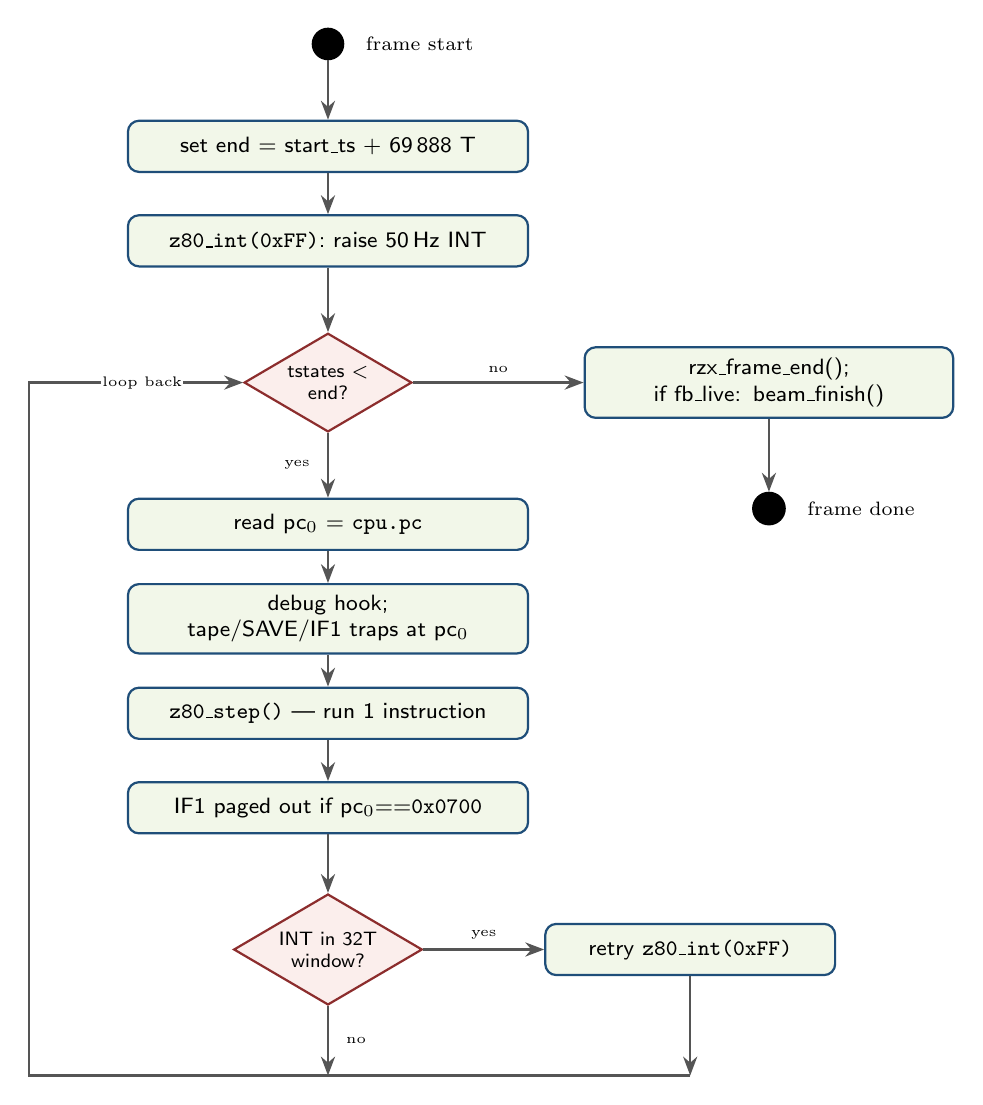
\begin{tikzpicture}[font=\sffamily\footnotesize]
  % --- spine (x = 0): actions and the two compact decision diamonds ---
  \node[actstart] (s)  at (0, 0.5) {};
  \node[right=1.5mm of s, font=\scriptsize] {frame start};
  \node[actnode, text width=48mm] (a0) at (0,-0.8) {set end = start\_ts + 69\,888 T};
  \node[actnode, text width=48mm] (a1) at (0,-2.0) {\texttt{z80\_int(0xFF)}: raise 50\,Hz INT};
  \node[actdec] (d1) at (0,-3.8) {tstates $<$\\end?};
  \node[actnode, text width=48mm] (a2) at (0,-5.6) {read pc$_0$ = \texttt{cpu.pc}};
  \node[actnode, text width=48mm] (a3) at (0,-6.8) {debug hook; tape/SAVE/IF1 traps at pc$_0$};
  \node[actnode, text width=48mm] (a4) at (0,-8.0) {\texttt{z80\_step()} --- run 1 instruction};
  \node[actnode, text width=48mm] (a5) at (0,-9.2) {IF1 paged out if pc$_0$==\texttt{0x0700}};
  \node[actdec] (d2) at (0,-11.0) {INT in 32T\\window?};

  % --- right side: exit + retry detour ---
  \node[actnode, text width=44mm] (a7) at (5.6,-3.8)
        {rzx\_frame\_end();\\ if fb\_live: beam\_finish()};
  \node[actfinal] (f1) at (5.6,-5.4) {};
  \node[right=1.5mm of f1, font=\scriptsize] {frame done};
  \node[actnode, text width=34mm] (a6) at (4.6,-11.0) {retry \texttt{z80\_int(0xFF)}};

  % --- spine flows ---
  \draw[actflow] (s)  -- (a0);
  \draw[actflow] (a0) -- (a1);
  \draw[actflow] (a1) -- (d1);
  \draw[actflow] (d1) -- node[left,font=\tiny,xshift=-1mm]{yes} (a2);
  \draw[actflow] (a2) -- (a3);
  \draw[actflow] (a3) -- (a4);
  \draw[actflow] (a4) -- (a5);
  \draw[actflow] (a5) -- (d2);

  % --- d1 "no" exits right to a7/final (bypasses the body) ---
  \draw[actflow] (d1.east) -- node[above,font=\tiny]{no} (a7.west);
  \draw[actflow] (a7) -- (f1);

  % --- d2 branches: yes->retry(a6), no->direct; both join the bottom rail ---
  \draw[actflow] (d2.east) -- node[above,font=\tiny]{yes} (a6.west);
  \draw[actflow] (d2.south) -- node[right,font=\tiny,xshift=1mm]{no} (0,-12.6);
  \draw[actflow] (a6.south) -- (4.6,-12.6);

  % --- single loop-back rail up the LEFT margin (clear of all boxes) ---
  \draw[actflow] (4.6,-12.6) -- (-3.8,-12.6) -- (-3.8,-3.8) -- (d1.west)
        node[pos=0.80,left=2mm,font=\tiny,fill=white,inner sep=0.5pt]{loop back};
\end{tikzpicture}
\caption{Activity Diagram of one emulated frame. Three properties matter:
\textbf{(1) drift-free}---frame boundaries are exact multiples of 69{,}888 T
(overshoot carries forward); \textbf{(2)} the INT window is the real $\sim$32 T;
\textbf{(3)} ROM traps and IF1 paging are PC predicates evaluated before each step.}
\end{figure}

% ============================================================
\section{Beam-accurate video (\texttt{src/video.c})}

Rather than rendering once per frame, the display is \textbf{painted
incrementally at the beam position}, so mid-frame effects are correct.

\begin{figure}[h]\centering
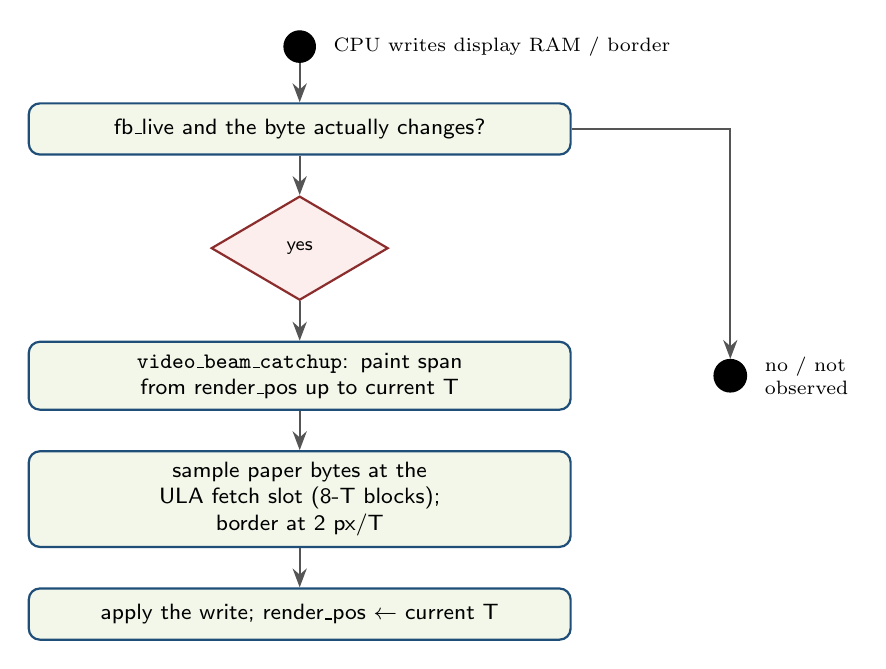
\begin{tikzpicture}[node distance=5mm]
  \node[actstart] (s) {}; \node[right=1mm of s,font=\scriptsize] {CPU writes display RAM / border};
  \node[actnode, below=of s, text width=66mm, align=center] (a1)
        {fb\_live and the byte actually changes?};
  \node[actdec, below=of a1, text width=16mm] (d1) {yes};
  \node[actnode, below=of d1, text width=66mm, align=center] (a2)
        {\texttt{video\_beam\_catchup}: paint span from render\_pos up to current T};
  \node[actnode, below=of a2, text width=66mm, align=center] (a3)
        {sample paper bytes at the ULA fetch slot (8-T blocks);\\ border at 2 px/T};
  \node[actnode, below=of a3, text width=66mm, align=center] (a4)
        {apply the write; render\_pos $\leftarrow$ current T};
  \node[actfinal, right=18mm of a2] (f) {};
  \node[right=1mm of f,font=\scriptsize,align=left] {no / not\\observed};
  \draw[actflow] (s) -- (a1);
  \draw[actflow] (a1) -- (d1);
  \draw[actflow] (d1) -- node[font=\tiny,right]{} (a2);
  \draw[actflow] (a2) -- (a3);
  \draw[actflow] (a3) -- (a4);
  \draw[actflow] (a1) -| (f);
\end{tikzpicture}
\caption{Activity Diagram of the lazy catch-up painter. Painting is gated on
\texttt{fb\_live}: turbo/headless runs that nobody observes skip it entirely
(\texttt{main.c} sets \texttt{fb\_live=(f==frames-1)}). \texttt{paint\_cell()}
also models \textbf{ULA snow}: with \texttt{I} in \texttt{0x40-0x7F} the low 7
bits of the fetch address come from \texttt{R}. \texttt{video\_screen\_text()}
does \textbf{ROM-font OCR} (match each 8$\times$8 cell against the font at
\texttt{0x3D00})---how the test suite asserts on screen contents without image
diffing.}
\end{figure}

% ============================================================
\section{Tape subsystem (\texttt{src/tape.c})}

Two loading paths share one pulse stream:

\begin{itemize}
\item \textbf{Trap loading} (default, instant): when PC hits \texttt{0x0556}
      (LD-BYTES), \texttt{tape\_trap()} copies the next block straight into RAM.
\item \textbf{Pulse loading} (\texttt{-{}-real-tape}): the whole tape is
      compiled at load time into a flat list of pulse durations
      (\texttt{tape.c:33}) using standard ROM timings; EAR toggles per edge
      against the cycle-exact clock (\texttt{tape\_player\_ear},
      \texttt{tape.c:700}).
\end{itemize}

Formats: \texttt{.tap} (raw), \texttt{.tzx} (turbo, CSW \texttt{0x18}
RLE$+$zlib, generalized-data \texttt{0x19}), sampled \texttt{.wav}
(DC removal + Schmitt trigger, 4--192\,kHz). \texttt{SAVE} is trapped at
\texttt{0x04C2} (SA-BYTES) and captured byte-exact to \texttt{.tap}.

\subsection{Tape player state machine}
The player's pause/resume logic at block boundaries is what makes multi-load
schemes ("stop the tape / press any key", rewind prompts) work without a UI.
The figure below models that behaviour.

\begin{figure}[h]\centering
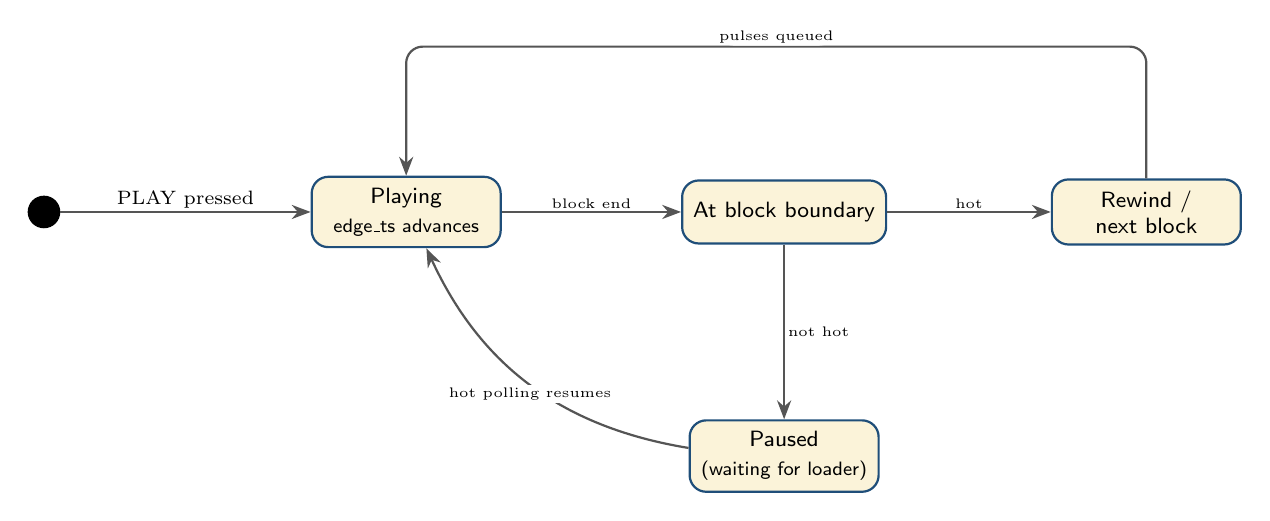
\begin{tikzpicture}[font=\sffamily\footnotesize]
  % states laid out left-to-right with generous gaps; pause below the boundary
  \node[smstart] (s)     at (0,0)    {};
  \node[smstate] (play)  at (4.6,0)  {Playing\\[1pt]\scriptsize edge\_ts advances};
  \node[smstate] (bound) at (9.4,0)  {At block boundary};
  \node[smstate] (rew)   at (14.0,0) {Rewind /\\next block};
  \node[smstate] (pause) at (9.4,-3.1) {Paused\\[1pt]\scriptsize (waiting for loader)};

  % transitions (every label white-filled so it never sits on a line)
  \draw[smflow] (s) -- node[above,font=\scriptsize,fill=white,inner sep=1pt]{PLAY pressed} (play);
  \draw[smflow] (play)  -- node[above,font=\tiny,fill=white,inner sep=1pt]{block end} (bound);
  \draw[smflow] (bound) -- node[above,font=\tiny,fill=white,inner sep=1pt]{hot} (rew);
  \draw[smflow] (bound.south) -- node[right,font=\tiny,fill=white,inner sep=1pt]{not hot} (pause.north);
  \draw[smflow] (pause) to[bend left=28] node[below,font=\tiny,fill=white,inner sep=1pt]{hot polling resumes} (play);
  % pulses queued: routed over the top, clear of all other arrows
  \draw[smflow, rounded corners=6pt] (rew.north) -- (14.0,2.1)
        -- node[above,font=\tiny,fill=white,inner sep=1pt]{pulses queued} (4.6,2.1)
        -- (play.north);
\end{tikzpicture}
\caption{State-Machine Diagram of the pulse player. \emph{Hot} = $\geq$32 EAR
reads per 10{,}000-T window, excluding the ROM keyboard scanner
(\texttt{0x028E-0x02BE}). \texttt{-{}-tape-b} + \texttt{tape\_swap()} model a
second cassette side.}
\end{figure}

% ============================================================
\section{Disk \& CP/M (\texttt{src/fdc.c}) --- HC-2000}

A polled uPD765/i8272 emulation: FDC at \texttt{0x85}/\texttt{0x87} with a
control latch at \texttt{0x05/0x07} (TC, drive select, reset). Implemented
commands: SPECIFY, SENSE DRIVE/INTERRUPT STATUS, RECALIBRATE, SEEK, READ ID,
READ/WRITE DATA (multi-sector, TC/EOT terminated), FORMAT TRACK; unknown
commands return the invalid ST0. Seeks are instantaneous; transfers are
byte-polled through MSR RQM/DIO. Raw \texttt{.img}/\texttt{.dsk} images in the
four period geometries (640K/720K 80-track, 320K/360K 40-track) are recognised
by size; dirty images write back at exit. Together with the HC-2000 memory map
(\S6) this boots \textbf{CP/M 2.2 from the system tracks to the \texttt{A>}
prompt} with working \texttt{DIR}.

% ============================================================
\section{State: snapshots \& RZX}

\textbf{Snapshots} (\texttt{src/snapshot.c}): read/write for \texttt{.sna}
(48K), \texttt{.z80} v1/v2/v3 (48K and 128K mode 3, pages 3--10; v1 RLE),
\texttt{.szx} (zx-state v1.4, with \textbf{zlib-compressed RAM pages} loaded
through the built-in \texttt{inflate.c}), raw \texttt{.scr}. HALT state survives
saving by re-pointing PC at the HALT opcode (\texttt{snapshot.c:56}).

\textbf{RZX} (\texttt{src/rzx.c}) is a record/replay pair for deterministic
whole-session regression. The sequence diagram below shows the replay contract.

\begin{figure}[h]\centering
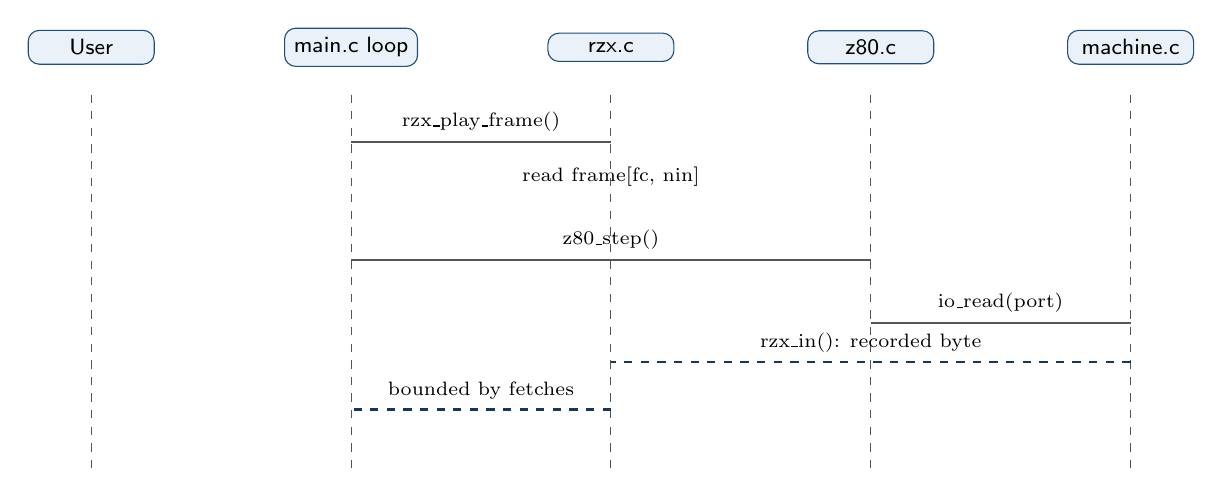
\begin{tikzpicture}[font=\footnotesize\sffamily]
  % lifelines (compressed to fit text width)
  \foreach \x/\n in {0/User, 3.3/{main.c loop}, 6.6/{rzx.c}, 9.9/{z80.c}, 13.2/machine.c} {
    \node[draw=accent,fill=blockfill,rounded corners,minimum width=16mm] at (\x,0) {\n};
    \draw[dashed,linegray] (\x,-0.6) -- (\x,-5.4);
  }
  % messages
  \draw[assoc,-] (3.3,-1.2) -- node[above,font=\scriptsize]{rzx\_play\_frame()} (6.6,-1.2);
  \draw[assoc,-] (6.6,-1.9) -- node[above,font=\scriptsize]{read frame[fc, nin]} (6.6,-1.9);
  \draw[assoc,-] (3.3,-2.7) -- node[above,font=\scriptsize]{z80\_step()} (9.9,-2.7);
  \draw[assoc,-] (9.9,-3.5) -- node[above,font=\scriptsize]{io\_read(port)} (13.2,-3.5);
  \draw[depends,-] (13.2,-4.0) -- node[above,font=\scriptsize]{rzx\_in(): recorded byte} (6.6,-4.0);
  \draw[depends,-] (6.6,-4.6) -- node[above,font=\scriptsize]{bounded by fetches} (3.3,-4.6);
\end{tikzpicture}
\caption{Sequence Diagram: during RZX playback, port reads are fed from the
recording. Frames are bounded by the \texttt{fetches} counter (bumped on every
R increment), so a captured session replays bit-exactly. Recording embeds a
\texttt{.z80} snapshot at start.}
\end{figure}

% ============================================================
\section{Input, debugger, frontend, CLI}

\textbf{Input} (\texttt{src/keys.c}): \texttt{keys\_apply(frame)} materialises
the 8-row keyboard matrix from \texttt{KeyEvent} ranges each frame. Three input
modes build them: \texttt{keys\_type} (types a BASIC string with keyword/symbol
composition), \texttt{keys\_raw} (a raw chord by name), \texttt{keys\_joy}
(joystick routed by \texttt{-{}-joy-type} to Kempston/Sinclair/cursor).
Kempston is gated behind \texttt{-{}-kempston} because an \emph{absent}
interface must leave \texttt{0x1F} floating.

\textbf{Disassembler} (\texttt{src/disasm.c}): full-coverage, decoded
algorithmically by the x/y/z/p/q bit fields rather than a 256-entry table, so
all prefixes, undocumented result-copy forms, ED no-ops and dead prefixes are
uniform. Locked by \texttt{tests/dtest.c} (124 cases).

\textbf{Monitor} (\texttt{src/debug.c}): PC breakpoints, memory read/write and
I/O-port watchpoints (each $\leq$32), single-step, hex dump, registers with
frame-relative T-state, per-instruction trace-to-file. Scriptable via
\texttt{-{}-debug "regs;step 3;cont"} then stdin (auto-continues when both are
exhausted so headless runs never hang). The \texttt{debug\_note\_*} hooks arm a
stop that fires before the next instruction---clean separation from the
timing-critical core.

\textbf{SDL frontend} (\texttt{src/sdl.c}): the standout choice---SDL2 is
\texttt{dlopen}'d at runtime and a minimal ABI slice declared in-tree, so the
build needs no SDL headers or link libraries. Features: resizable window,
\textbf{audio-clocked 50\,Hz pacing} (20\,ms tick fallback), full
host-keyboard$\to$matrix map, first game controller $\to$ Kempston,
turbo/pause/quit, quick save/load, fullscreen, drag-and-drop file loading.

\textbf{CLI} (\texttt{src/main.c}): $\sim$520-line option parser/orchestrator.
ROM path resolution (\texttt{main.c:74}) prefers the relative path (in-tree)
and falls back to \texttt{HC91\_DATADIR} (\texttt{/usr/share/hc91emu}).

% ============================================================
\section{Testing \& validation}

\begin{center}\footnotesize
\begin{tabular}{@{}p{2.6cm}p{5.0cm}p{7.8cm}@{}}
\toprule
\textbf{Layer} & \textbf{What} & \textbf{How} \\
\midrule
CPU unit      & T-state totals, contention M-cycles, disassembly & \texttt{ttest/ctest/dtest} --- pure, no ROMs \\
CPU exerciser & documented + undocumented flags & \texttt{zexrun} runs \texttt{zexdoc/zexall.com} \\
CPU vectors   & full per-instruction bus traces & \texttt{sst} replays 162 SingleStepTests files (162{,}000) \\
In-machine    & Rak's z80full/ccf/memptr & loaded as tapes; screen asserts ``all tests passed'' \\
Integration   & boot, BASIC, games, audio, tape, disk, CP/M, SDL & golden PNGs + OCR + WAV pitch \\
\bottomrule
\end{tabular}
\end{center}

Key ideas: generated \texttt{.tap} files (\texttt{bordertap.c},
\texttt{multitap.c}) produce \emph{known} beam effects to lock the renderer;
\texttt{-{}-text} OCR avoids image-diff fragility; \texttt{-{}-fb-dump} +
\texttt{fbcheck.c} do pixel-exact checks; RZX gives bit-exact whole-session
regression. \textbf{CI} runs only the download-free subset (no ROMs, no
copyrighted data, no network): build + \texttt{ttest/ctest/dtest/zexdoc},
repeated under \textbf{ASan + UBSan}.

% ============================================================
\section{Notable engineering decisions}

\begin{enumerate}
\item \textbf{Bus-callback CPU core} (\texttt{z80.c})---the single most
      important abstraction: makes the core reusable (\texttt{zexrun}),
      testable in isolation, and decouples timing accuracy from machine specifics.
\item \textbf{Incremental per-M-cycle T-state accounting} with contention
      evaluated at access time---the foundation making contention, floating bus
      and beam video all cycle-exact simultaneously.
\item \textbf{Zero external dependencies}---a hand-written DEFLATE inflater,
      PNG encoder and SDL ABI slice keep the build trivial and the binary
      self-contained.
\item \textbf{\texttt{dlopen} SDL} instead of a build-time dependency---headless
      stays the default, tests need no display, one \texttt{make} target builds all.
\item \textbf{One aggregate \texttt{Machine} struct, no globals}---clean
      ownership, easy to reset/snapshot/reason about.
\item \textbf{Drift-free frame loop} (exact 69{,}888-T boundaries, overshoot
      carried forward) keeps phase locked indefinitely.
\item \textbf{Test-tape generation + OCR assertion} instead of brittle image
      diffs---deterministic and human-readable.
\item \textbf{Going beyond MAME}: MAME's \texttt{hc91} driver is a plain ROM
      swap; this emulator implements the actual CP/M paging, the HC-128's genuine
      banking+AY (confirmed by disassembling its ROM), and the HC-2000's full
      disk interface + CP/M boot.
\end{enumerate}

\vspace{2pt}\hrule height 0.4pt
\begin{center}\footnotesize
Source under the MIT License; the grant covers the emulator only---ROMs and
period software are never committed and are fetched on demand by
\texttt{tools/get\_roms.sh}. Derived from a source audit of the
\texttt{cosmindxu/hc91emu} tree ($\sim$7{,}700 lines of C99).
\end{center}

\end{document}
